\subsection{研究報告(松島 慎)}
本節では松島研究室の研究活動について報告する。
2019年度および2020年度に、弊研究室では解釈可能な機械学習手法の効率的な計算手法についての研究を推進してきた。

大量のデータから複雑な関数を推定することにより画像データや言語データを予測したり生成したりするなど、表層的に駆使することは可能になってきた。
しかしながら我々の画像や言語に対する理解が進んだわけではない。現代社会には様々なデータがあり、データを上記の意味で駆使するだけでなく、データの隠れた法則性や生成原理などの理解に結び付く属性間の関係を抽出することが求められる。

機械学習は予測や分類など表層的なデータの駆使の方法論であるだけでなく、
データの関係を明らかにして人間の理解を助けるための方法論でもあり、
特にデータ保持者がデータを理解するのに有用なモデルとして以下の3つの分野に関する研究を行った。
\begin{itemize}
    \item 一般化加法モデルに関する研究
    \item 組合せ線形モデルに関する研究
    \item 部分空間クラスタリングに関する研究
\end{itemize}

一般化加法モデルと組み合わせ線形モデルは
属性間の線形な関係を越えて、非線形な関係を抽出するための枠組みである。
部分空間クラスタリングはデータ集合が持つ単純な線形関係を超えて、
データのクラスタリングを行ってそれぞれのクラスタが持つ線形関係を抽出する枠組みである。


\subsubsection{一般化加法モデルに関する研究}
教師あり学習の文脈において、線形モデルの学習とは以下のようにあらわされるデータの属性間の線形な関係を抽出する枠組みととらえることができる:
\begin{align*}
    y = \sum_{j=1}^d w_j x_j.
\end{align*}
データの属性$y$は通常予測したい変数であり、
予測のために用いられるデータの他の属性が$x_j$であらわされる($j=1,\ldots,d$)。与えられたデータ集合を用いて各$w_j$は実数全体から推定される。
一般化加法モデル\cite{F}は線形モデルと同様に以下のような関係を抽出する枠組みである:
\begin{align*}
    y = \sum_{j=1}^d f_j (x_j).
\end{align*}
このとき、与えられたデータ集合を用いて各$f_j$は(十分広い)関数クラス$F$から推定される。
このような$f_j$を推定できれば、例えば年齢と収入の非線形な関係などがデータから学習できると考えられる。

最も単純な手法は$F$を推定の簡単さのために狭めの関数クラスに制限することである。一般に与えられた基底関数集合$\left\{\varphi_k:\mathbb{R} \to \mathbb{R} \right\}_{k=1,\ldots,K}$に対し
\begin{align*}
  F=\left\{  \sum_{j=1}^d\sum_{k=1}^{K} w_{kj}\varphi_k(x_j) \right\}
\end{align*}
とすれば、通常の線形モデルの学習と同様に学習が可能であるが、
基底関数たち$\phi_k$と$d'$をデータに応じてうまく選ぶ必要がある。このような方法はパラメトリックな手法と呼ばれる。

利用可能なデータ数に応じて関数クラスの大きさが変わる。
具体的にはデータ数が大きくなれば関数クラスも広くなっていくような手法をノンパラメトリックな手法と呼ぶ。
ノンパラメトリックな手法では各$f_j$は以下のように表される無限次元の空間$F$から推定されると考えることができる:
\begin{align*}
    F = \{f | \|f\|\le C\}
\end{align*}
ここで$\|\cdot\|$はある関数空間上で定義されたノルムである。上述のような手法はカーネル法を使うよりなかった。
我々の手法はカーネル法よりも効率的に学習が可能である。

さらに対象の属性が二変数関数$f_{j,k}(x_j,x_k)$の和で表されるような複雑な関係性をデータから学習して可視化することを考える。すなわち、以下の以下のような$y$と$x$の関係を抽出することを考える:
\begin{align*}
    y = \sum_{j,k} f_{j,k} (x_j,x_k)
\end{align*}
ここでデータから$f_{j,k}$を$F$から推定する。
\cite{KM01}、\cite{KM02}では二変数関数の空間に対して
二変数全変動ノルムを新しく定義し、これに基づく定式化および推定のための最適化アルゴリズムを提案した。さらに計算機実験において既存手法に比べより正確に真の関数を推定できることを示した。
\begin{figure*}[h]
    \centering
    \begin{tabular}{c}
        \begin{minipage}{0.04\hsize}
            \centering
        \end{minipage}
        \begin{minipage}{0.24\hsize}
            \centering
            Ground Truth
        \end{minipage}
        \begin{minipage}{0.24\hsize}
            \centering
            Proposed
        \end{minipage}
        \begin{minipage}{0.24\hsize}
            \centering
            $\rm GA^2M$
        \end{minipage}
        \begin{minipage}{0.24\hsize}
            \centering
            pyGAM
        \end{minipage}
        \\ \hline
        \begin{minipage}{0.04\hsize}
            \small
            $x_0, x_1$
        \end{minipage}
        \begin{minipage}{0.24\hsize}
            \centering
            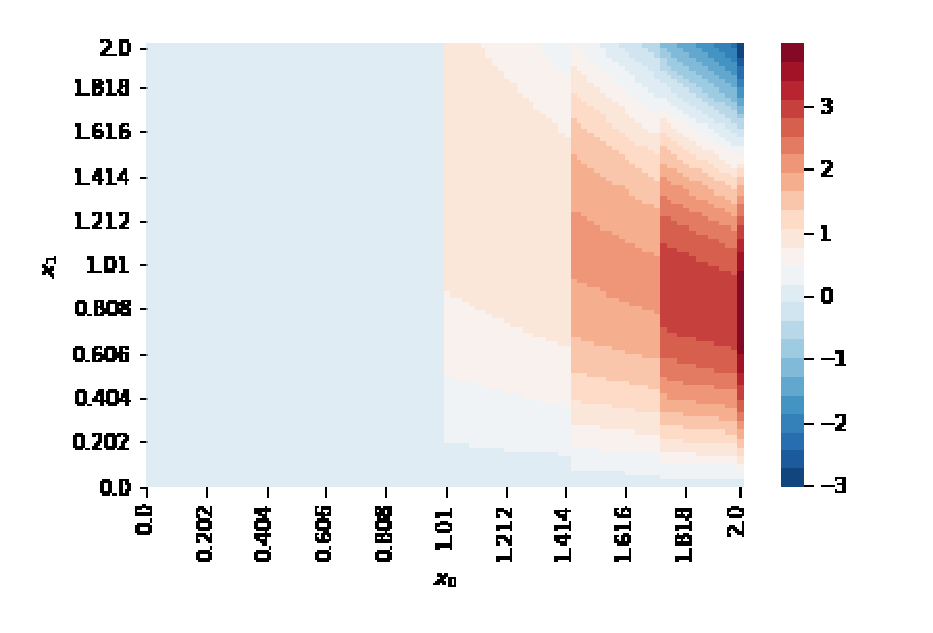
\includegraphics[width=0.95\hsize]{Matsushima/heatmaps/ideal-01.eps}
            % 理論値:$x_0 x_1$
        \end{minipage}
        \begin{minipage}{0.24\hsize}
            \centering
            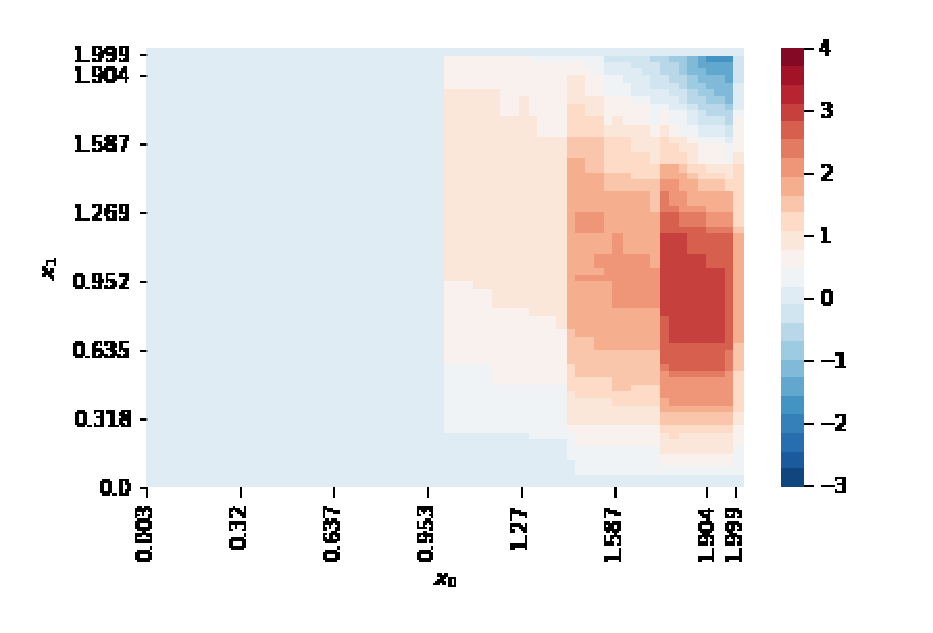
\includegraphics[width=0.95\hsize]{Matsushima/heatmaps/tvgam-01.eps}
            % IGAMの学習した相互作用
        \end{minipage}
        \begin{minipage}{0.24\hsize}
            \centering
            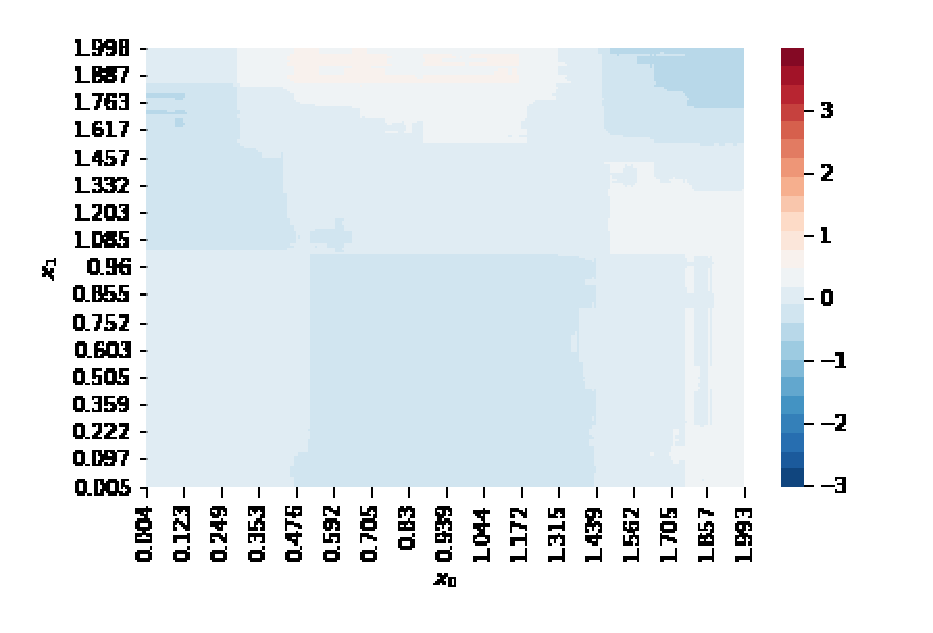
\includegraphics[width=0.95\hsize]{Matsushima/heatmaps/mltk-01.eps}
            % $\rm GA^2M$の学習した相互作用
        \end{minipage}
        \begin{minipage}{0.24\hsize}
            \centering
            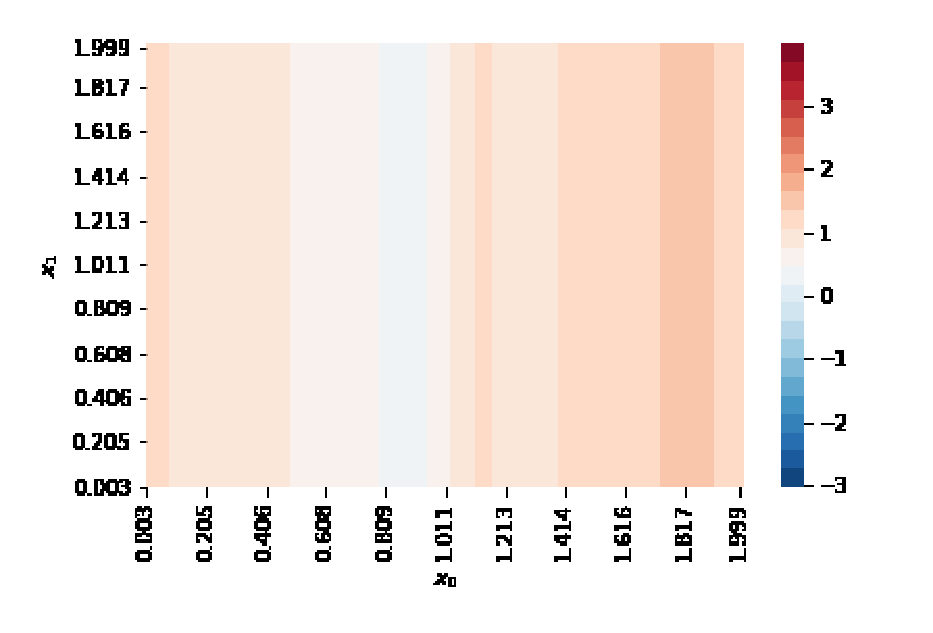
\includegraphics[width=0.95\hsize]{Matsushima/heatmaps/pygam-01.eps}
        \end{minipage}
    \end{tabular}
    \caption{人口データを用いた提案手法と既存手法($\rm GA^2M$およびpyGAM)の推定した二変数相互作用を表す関数の様子。Ground Truthは訓練データを生成した真の関数。}
\label{fig:heatmap-comparison-synthetic-data-2}
\end{figure*}

\subsubsection{組合せ線形モデルに関する研究}

組合せ線形モデルでは離散データ集合を考える。
実用的なデータの属性は例えば性別など示量的に表せないことも多く、このような属性の集合は通常離散データ、すなわち$\{0,1\}^n$上のデータとして扱われることが多い。
このよ8うな離散的な属性を複数持つようなデータを考えると、属性間の相互作用の数はデータの属性数に対して指数的に増加するため、離散データ空間での相互作用を扱う効率的な学習方法を発明することは重要である。

 前述の目的のためにイジングモデルやボルツマンマシンのような無向グラフィカルモデルと言われるモデルがよく用いられる。これらのモデルは二次までの相互作用しか扱えないのに対して、高次元対数線形モデルはデータ間のより高次元の相互作用を表現することが可能である。また、高次元対数線形モデルはフィッシャー情報量とe-接続とm-接続に基づく双対平坦構造を持つことから、理論的にも重要である。
 
高次対数線形モデルは
\begin{align*}
    \log P(x;\theta) = \sum_{\phi\in B} \theta_\phi \phi(x)  - \log\left( \sum_{x'\in S} \exp\left( \sum_{\phi\in B} \theta_\phi \phi(x') \right) \right)    
\end{align*}
と表される。ここで$\phi \in B \subset \{0,1\}^n$と$\phi:\{0,1\}^n\to \{0,1\} $を同一視する。すなわち$\phi(x)$の値を以下で定義する。
\begin{align*}
    \phi(x)  = \begin{cases}
    1 & 全ての j で \phi_j \le x_j, \\
    0 & 上記以外.
    \end{cases}
\end{align*}

\cite{LMY01}では、識別モデルにおいて教師あり学習を行う場合に効率的な学習アルゴリズムを提案した。実験によって論理結合による特徴は各説明変数が同時に真である場合の効果を表すと解釈できるため、解釈性も予測性能も高い予測が可能であることを示した。
行う。

さらに本研究では生成モデル、すなわち二値データの分布の推定問題も対象とした。教師なし学習の文脈では、与えられたデータの特徴を解釈可能であり、かつ真の分布をよく近似する分布を推定することを目指す。
本研究では自然スパース性(Natural Sparsity, Natural Sparseness)という概念を導入し、より自然スパース性が高いモデルを推定するような定式化と方法論を提案する。

本研究で対象とするデータ$D\subset\{0,1\}^n$を生成する確率分布は、ある$D\subset S\subset\{0,1\}^n$なる$S$に対して、以下の集合$M$の元であるとする。
\begin{align*}
    M = \left\{ P(\cdot)\middle| 0<P(x)<1, \sum_{x\in S} P(x) = 1 \right\}
\end{align*}
$M$には双対平坦な座標系が存在し、それぞれの座標系での値を
自然パラメータ$\theta \in \mathbb{R}^{|S|}$
と期待パラメータ$\eta \in \mathbb{R}^{|S|}$で表す。

これらのパラメータは$\mathbb{R}^{2^n}$の空間へ拡張して考えることができる。自然パラメータの場合、$M$の要素である確率分布を表す$\theta \in \mathbb{R}^{|S|}$は唯一であるが、同じ要素を表すパラメータ$\theta \in \mathbb{R}^{2^n}$は複数存在する。
$M$の元であるところの確率分布に対し自然スパース性とは、対象の確率分布を表す複数の$\theta\in\mathbb{R}^{2^n}$のうち最も非零要素が少ないパラメータの非零要素の数とする。
すなわち$P\in M$に対し以下のように定義する。
\begin{align*}
    {\rm NS}(P) =  \min_{\theta\in \mathbb{R}^{2^n}, P = P(\cdot;\theta)} \|\theta\|_0
\end{align*}
一方で期待パラメータ$\eta$は$\mathbb{R}^{|S|}$の元としても$\mathbb{R}^{2^n}$の元としても唯一である。

非零要素を多く含む自然パラメータで表される確率分布は単純で扱いやすい分布であり、例えば単純な対数線形モデルやイジングモデルは高次の$\theta$の値を0に制限したモデルである。
一方で、任意の分布に関して$\eta$はスパース性はない。すなわち、任意の分布で混合パラメータの値は正の値である。


\cite{HSM01}、\cite{HSM02}ではこのような意味でスパースなモデルの学習が座標降下法により効率的に学習可能であることを示した。


\subsubsection{部分空間クラスタリングに関する研究}

部分空間クラスタリングとは複数の低次元空間にデータをクラスタリングする手法である。通常のクラスタリング手法では距離的に近いデータの集まりをクラスタとみなす。一方で、部分空間クラスタリングでは同じ低次元空間にあるデータをクラスタとみなす(図~\ref{fig:my_label}を参照)。画像データや文章データなどはタスクによって部分空間クラスタリングをした方がよいということが2011年VIDAL\cite{SC}によって提案されて以降、多くの部分空間クラスタリング手法が開発されている。

\begin{figure}[h]
    \centering
    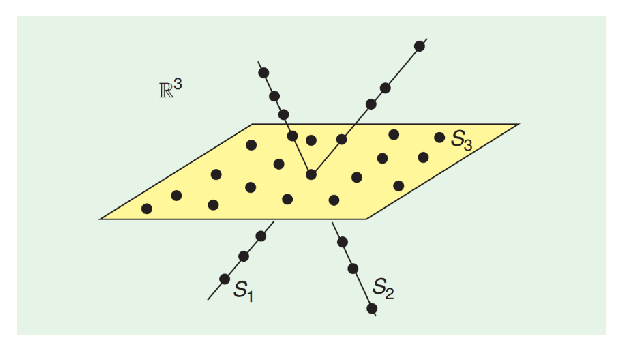
\includegraphics[width=7cm]{Matsushima/sc.eps}
    \caption{部分空間クラスタリングの3次元の例(\cite{SC}から抜粋)。距離が近い点同士ではなく、同じ平面上もしくは同じ直線上(部分空間上)にある点同士をクラスタとみなす。}
    \label{fig:my_label}
\end{figure}
\cite{NM01}は〜

\begin{thebibliography}{9}
\bibitem{F}
    Friedman, J., Hastie, T., & Tibshirani, R. (2010). 
    Applications of the lasso and grouped lasso to the estimation of sparse graphical models (pp. 1-22). Technical report, Stanford University.
\bibitem{SC}
 VIDAL, René. Subspace clustering. IEEE Signal Processing Magazine, 2011, 28.2: 52-68.
\end{thebibliography}

